
% This LaTeX was auto-generated from MATLAB code.
% To make changes, update the MATLAB code and republish this document.

\documentclass{article}
\usepackage{graphicx}
\usepackage{color}

\sloppy
\definecolor{lightgray}{gray}{0.5}
\setlength{\parindent}{0pt}

\begin{document}

    
    
\subsection*{Contents}

\begin{itemize}
\setlength{\itemsep}{-1ex}
   \item Part 1
   \item Part 2
\end{itemize}


\subsection*{Part 1}

\begin{par}
Using the derivation given in the book, we will derive the Frequency Response Functions for particular solution cos(wt).
\end{par} \vspace{1em}
\begin{verbatim}
clear

f = linspace(2,500,1024);
g = linspace(0,pi,1024);
Re_y = (1-g.^-2)./(g.^-4 - 1.9999*g.^-2 + 1);
Im_y = 0.01*(g.^-1)./(g.^-4 - 1.9999*g.^-2 + 1);
Mag_y = sqrt(Re_y.^2+Im_y.^2);
C_i = Mag_y;
phase = atan2(Im_y,Re_y);
frf1 = Re_y + 1i*Im_y;
semilogy(g./(2*pi),C_i);
xlabel('Hz (1/s)')
ylabel('|FRF|')


grid on;
figure;
plot(g./(2*pi),phase*45);
xlabel('Hz (1/s)')
ylabel('angle(FRF)')
grid on;
\end{verbatim}

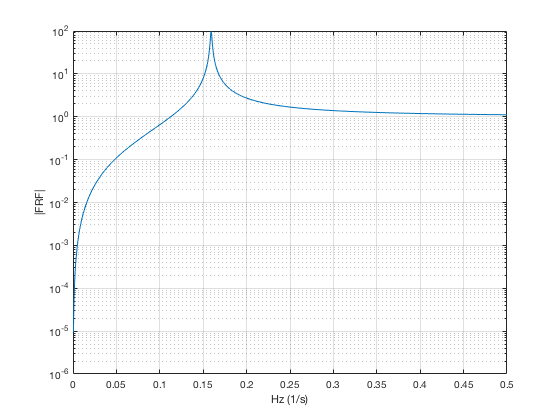
\includegraphics [width=4in]{HW2_01.eps}

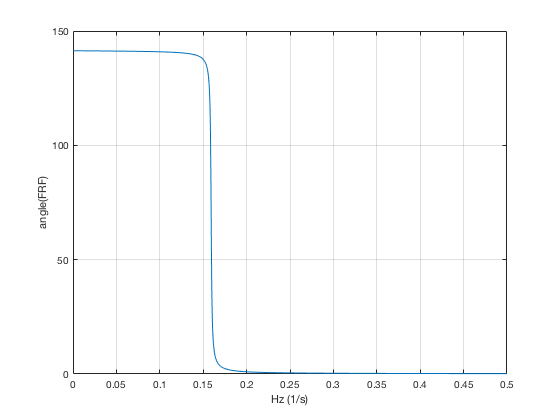
\includegraphics [width=4in]{HW2_02.eps}


\subsection*{Part 2}

\begin{par}
We will obtain the same FRF now by system identification using a set of input-output data. In particular, we will produce the same plots as above.
\end{par} \vspace{1em}
\begin{verbatim}
A_c = [
    0 1
    -1 -0.01
    ];
B_c = [0;1];
C_c = [-1 -0.01];
D_c = 1;
dt = 1; % seconds
syst = c2d(ss(A_c,B_c,C_c,D_c),dt);
A = syst.A;
B = syst.B;
C = syst.C;
D = syst.D;




n = 1024;
inp = randn(1,n);
inp(n/2:end) = 0;
%close ALL
figure

plot(inp)
x0 = [0.5;0.5];
[Y, X] = dlsim(A,B,C,D,inp,x0);

fft_o = fft2(Y');
fft_i = fft2(inp);

frf = fft_o./fft_i;
frf = frf(1:end/2);
semilogy(linspace(0,length(frf)/n,length(frf)),abs(frf));
xlabel('Hz (1/s)')
ylabel('|FRF|')
grid on
figure
plot(linspace(0,length(frf)/n,length(frf)),angle(frf)*45)
xlabel('Hz (1/s)')
ylabel('angle(FRF)')
\end{verbatim}

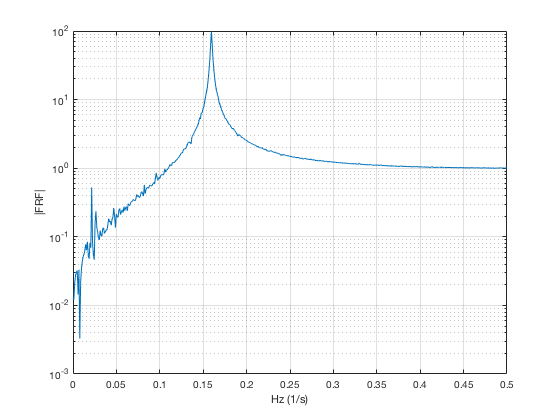
\includegraphics [width=4in]{HW2_03.eps}

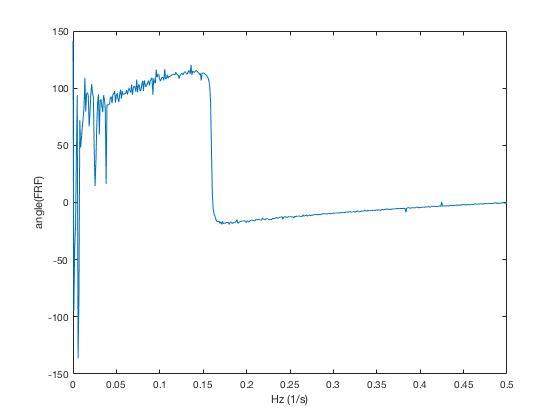
\includegraphics [width=4in]{HW2_04.eps}



\end{document}
    
